\documentclass[12pt,a4paper]{article}
\usepackage[polish]{babel}
\usepackage[T1]{fontenc}
\usepackage[utf8]{inputenc}
\usepackage{natbib}
\usepackage{graphicx}
\usepackage{indentfirst}
\usepackage[]{algorithm2e}
\usepackage{listingsutf8}
\usepackage{csquotes}
\lstset{
    inputencoding=utf8,
    language=Python, 
    escapeinside={\%*}{*)},
    breaklines=true,
    extendedchars=false,
}
\begin{document}
\title{Dokumentacja Egzaminu Praktycznego\\ Algorytmy i Struktury Danych}
\author{Konrad Lubera, gr IB}
\date{\today}

\maketitle

\newpage
\tableofcontents

\newpage
\section{Polecenie}
Temat 9: Napisz program/aplikację który/która: Wyznaczy listę słów, które pojawiają się w tekście z jednego pliku, a nie pojawiają się w tekście z pliku drugiego przy pomocy algorytmu Boyer-Moore.

\section{Algorytm}
\subsection{Opis}
Do wykonania zadania użyto, zgodnie z poleceniem algorytmu Boyera-Moorea. Jest to wersja która korzysta z funkcji bad-character shift, bardzo podobna do tej która zastała zaprezentowana na wykładzie. Polega na porównywaniu z prawej strony wzorca, jeżeli wzorzec nie będzie pasował, to algorytm przeskakuje o długość wzorca. Jest to bardzo szybki i efektywny algorytm ponieważ ilość porównań jest relatywnie mała. 
\BlankLine
Implementację wykonano w języku Python w wersji 3.8.
\subsection{Przykład działania}
\begin{figure}[h]
\centering
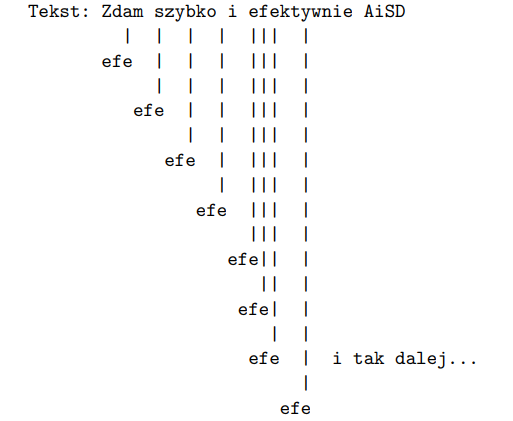
\includegraphics[scale=0.75]{przyklad.png}
\caption{Przykład działania algorytmu z notatek z wykładów}
\label{fig:przykład}
\end{figure}
\newpage

\subsection{Schemat blokowy}
\begin{figure}[h]
\centering
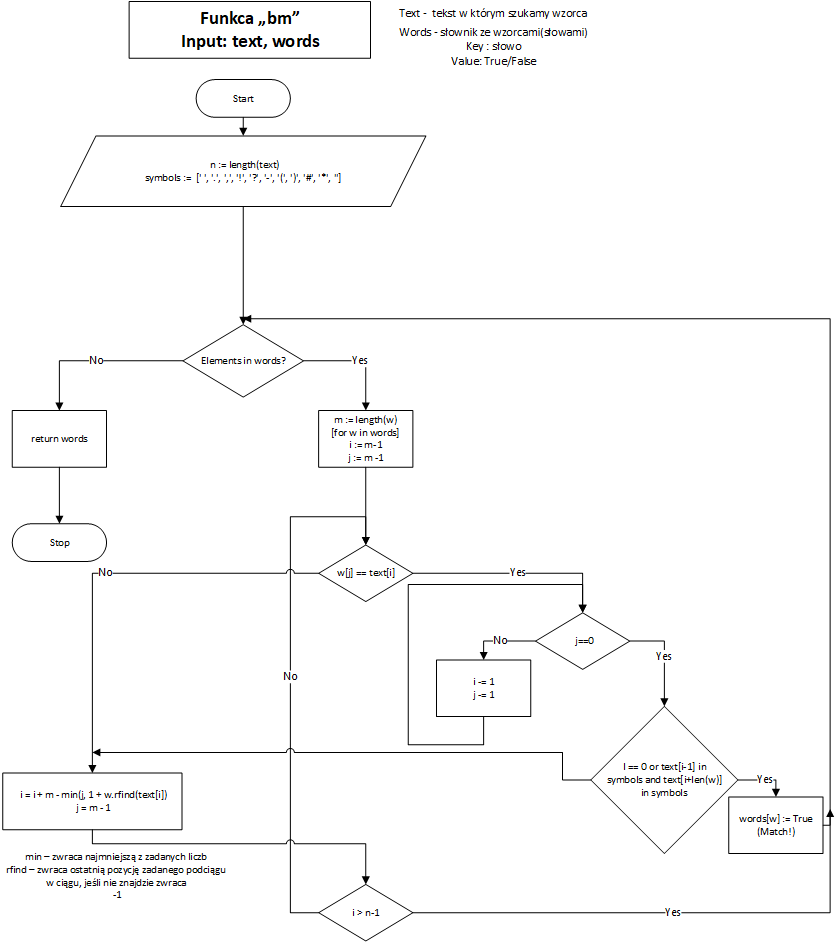
\includegraphics[scale=0.6]{boyermorre_flow.png}
\caption{Zastosowany algorytm Boyera Morrea}
\label{fig:boyer morre}
\end{figure}

\section{Opis rozwiązania}

\subsection{Napotkane problemy}
Podczas implementacji napotkano problem związany z tym, że algorytm służy, w jego oryginalnym wydaniu, do wyszukiwania fraz-wzorca co generuje problemy w wyszukiwaniu słów. Dla przykładu gdy naszym wzorcem jest słowo ,,dam'' a tekście mamy słowo ,,zdam'' algorytm uzna, że wzorzec się pojawił. Problem ten rozwiązano dojadając warunek który sprawdza czy znak przed i za dopasowaniem znajduje się na liście która zawiera znaki interpunkcyjne, często używane symbole oraz spację. Dodatkowo aby wyeliminować problem z dopasowanie słowa napisanego wielką literą i tego napisanego małą, wszystkie litery we wzorcu jak i tekście zostały zmienione na małe przy pomocy funkcji lower(). 

\subsection{Pseudokod}
\begin{algorithm}[H]
\SetKwInOut{Input}{input}\SetKwInOut{Output}{output}
\Input{$path$}
\Output{string $text$}
\BlankLine
open file on $path$  as $file$:\\
\hspace{2ex} $text$ = $file$.read\\
$text$ = lower($text$)\\
$file$.close\\
\Return{text}
\caption{Funkcja read to string\label{RS}}
\end{algorithm}

\BlankLine

\begin{algorithm}[H]
\SetKwInOut{Input}{input}\SetKwInOut{Output}{output}
\Input{$path$}
\Output{dictionary $words$}
\BlankLine
$words$:={}\\
$symbols$ := `.,!-?()"":'\\ 
open file on $path$  as $file$:\\
\hspace{2ex} \ForEach{$line$ in $file$}{
        \ForEach{$word$ in $line$}
        {
            $tmp$:=$word$.strip($symbols$)\\
            $tmp$ = lower($tmp$)\\
            \If{$tmp$ not in $words$ and $tmp$!=''}{
                    $words[tmp]$ = False \tcc*[r]{przypisanie do słownika}
                }
        }
}
\Return{$words$}
\caption{Funkcja read to dictionary\label{RD}}
\end{algorithm}

\begin{algorithm}[H]
\SetKwInOut{Input}{input}\SetKwInOut{Output}{output}
\Input{string $text$, dictionary $words$}
\Output{updated dictionary $words$}\
\BlankLine
$n$ := lenght($text$)\\
$symbols$ := [' ', '.', ',', '!', '?', '-', '(', ')', '*', '']\\
\ForEach{$w$ in $words$}{
$m$ := lenght($w$)\\
$j$ := $m$-1\\
$i$ := $m$-1\\
\Repeat{$i$>$n$-1}{
\eIf{$w[j]$==$text[i]$}
    {
        \eIf{$j$==0}
            {
                \eIf{$i$==0 or $text[i-1]$in$symbols$ and $text[i+len(w)]$in$symbols#$}
                    {
                        $words[w]$ = True \\
                        break
                    }
                    {
                        $i$ = $i$ + $m$ - min($j$, 1+ $w$.find($text[i]$))\\    
                        $j$ = $m$-1
                    }
            }
            {
                $i$ -= 1\\
                $j$ -= 1
            }
    }
    {
        $i$ = $i$ + $m$ - min($j$, 1+ $w$.find($text[i]$))\\    
        $j$ = $m$-1
    }}}
\Return {$words$}
\caption{Funkcja BM\label{BM}}
\end{algorithm}

\BlankLine
Pseudokod został napisany tylko dla funkcji które są ważne z punktu widzenia działania samego algorytmu.

\newpage
\section{Prezentacja wyników}
Teksty które zostały użyte do przetestowania programu zostały tak dobrane żeby sprawdzić czy problemy o których napisano w sekcji Algorytm - Opis zostały rozwiązane w rezultacie teksty mają dużo znaków interpunkcyjnych oraz słów które zawierają w sobie inne słowa. Teksy nie jest też zbyt długie żeby nie generować trudności podczas sprawdzania wyników, jednak przetestowano program używając dłuższych tekstów i też działa :D. 

Oto teksty:
\begin{itemize}
    \item file1.txt
    \begin{displayquote}
Byliśmy bardzo smutni, że nie mogliśmy wrócić na uczelnię, jednak najważniejsze było żeby przetrwać ten trudny czas pandemii i co najważniejsze dobrze napisać egzamin z algorytmów i struktur danych. Mam nadzieję ze to co zrobiłem wystarczy żebym zdał. Jeżeli nie będę bardzo zawiedziony! Kompletnie, nie, mam, pojęcia, jak, używać, znaków, interpunkcyjnych, więc, w, tym, zdaniu, przecinek, będzie, po, każdym, słowie. Umiejętności miękkie to nie jest moja mocna strona. Już nie wiem co tu napisać więc wkleję pierwszy akapit z Wikipedii o algorytmie Boyera Moore’a.
Algorytm Boyera i Moore'a algorytm poszukiwania wzorca w tekście. Polega na porównywaniu, zaczynając od ostatniego elementu wzorca.
\end{displayquote}
\item file2.txt
\begin{displayquote}
Byliśmy bardzo zawiedzeni, że w tym semestrze nie wrócimy już na uczelnię, jednak pomimo tego ucze (specjalnie błąd) się pilnie i dam z siebie wszystko. Mam nadzieję, że taki stan rzeczy nie będzie trwać w nieskończoność. Są ważniejsze sprawy od spotkania z kolegami np. egzamin z aisd który mimo trudności się obył w bardzo przystępnej formie. Nie będę tu już więcej pisać jakichś głupot tylko wkleję znów akapit z Wikipedii i kilka słów z generatora losowych słów ów. Algorytm Boyera i Moore'a algorytm poszukiwania wzorca w tekście. Polega na porównywaniu, zaczynając od ostatniego elementu wzorca. Rzeczownik, przestrzeń, biblioteka, rosa parks, szubienica, ośmiornica, wzmacniacz, atletyczny, farmaceuta, jeżozwierz, frustracja, bezradność, anne frank, niedźwiedź, rękawiczki, kierownica, studzienka, dominikana, ciężarówka, sprzedawca.
\end{displayquote}
\end{itemize}

To lista słów które pojawiają się w tekście z jednego pliku, a nie pojawiają się w tekście z pliku drugiego: \\ \\
\begin{minipage}[t]{0.3\textwidth}
\begin{enumerate}
\item Zawiedzeni
\item Semestrze
\item Wrócimy
\item Pomimo
\item Tego
\item Ucze
\item Specjalnie
\item Błąd
\item Się
\item Pilnie
\item Dam
\item Siebie
\item Wszystko
\item Taki
\item Stan
\item Rzeczy
\item Trwać
\item Nieskończoność
\item Są
\item Ważniejsze
\item Sprawy
\item Spotkania
\end{enumerate}
\end{minipage}
\begin{minipage}[t]{0.3\textwidth}
\begin{enumerate}
\setcounter{enumi}{22}
\item Kolegami
\item Np
\item Aisd
\item Który
\item Mimo
\item Trudności
\item Obył
\item Przystępnej
\item Formie
\item Więcej
\item Pisać 
\item Jakichś
\item Głupot
\item Tylko
\item Znów
\item Kilka
\item Słów
\item Generatora
\item Losowych
\item Ów
\item Rzeczownik
\item Przestrzeń
\end{enumerate}
\end{minipage}
\begin{minipage}[t]{0.3\textwidth}
\begin{enumerate}
\setcounter{enumi}{44}
\item Biblioteka
\item Rosa
\item Parks
\item Szubienica
\item Ośmiornica
\item Wzmacniacz
\item Atletyczny
\item Farmaceuta
\item Jeżozwierz
\item Frustracja
\item Bezradność
\item Anne
\item Frank
\item Niedźwiedź
\item Rękawiczki
\item Kierownica
\item Studzienka
\item Dominikana
\item Ciężarówka
\item Sprzedawca
\item Przeżyć
\item Samochód
\end{enumerate}
\end{minipage}
\newpage
Po wykonaniu programu otworzy się plik txt który zawiera ta listę oraz dodatkową statystykę. Jeżeli to nie nastąpi np gdy używamy systemu Linux wystarczy otworzyć plik ,,results.txt''. Istnieje możliwość zmiany tekstów na których operuje program wystarczy wyedytować zawartość plików ,,file1.txt'' i ,,file2.txt''. 
\BlankLine
\section{Kod programu}
\begin{lstlisting}
# -*- coding: utf-8 -*-
# Wyznaczy listę słów, które pojawiają się w tekście z jednego pliku, a nie pojawiają się w tekście z pliku drugiego przy pomocy algorytmu Boyer-Moore
import os


def read_to_string(path):
    with open(path, 'r', encoding="utf-8") as file:
        text = file.read()
    text = text.lower()
    text += " " # dodatkowe zabezpieczenie
    #print(text)
    file.close()
    return text


def read_to_dict(path):
    words = {}
    symbols = ' .,!-?()"":\n '  # warunki dla - w środku ! - strip załatwia sprwawe
    with open(path, 'r', encoding="utf-8") as file:
        for line in file:
            for word in line.split():
                tmp = word.strip(symbols)
                tmp = tmp.lower()
                # TYMCZASOWE ROZWIĄZANIE!
                #t = ' ' + tmp + ' '
                if tmp not in words and tmp != "":
                    words[tmp] = False
    # print("Ilość słów bez powtórzeń: " + str(len(words)))
    #print(words.keys())
    file.close()
    return words


def bm(text, words):
    n = len(text)
    symbols = [' ', '.', ',', '!', '?', '-', '(', ')', '#', '*', '']
    for w in words:
        m = len(w)
        i = m - 1
        j = m - 1
        while True:
            if w[j] == text[i]:
                if j == 0:
                    if i == 0 or text[i-1] in symbols and text[i+len(w)] in symbols:
                        words[w] = True
                        # print("Matched word: '" + w + "' on position: " + str(i))
                        # if i == 0:  print("Before: None")
                        # else: print("Before: " + text[i-1])
                        # print("After: " + text[i + len(w)])
                        break
                    else:
                        i = i + m - min(j, 1 + w.rfind(text[i]))
                        #i = i + m - min(j, 1 + w.rfind(text[i+len(w)]))
                        j = m - 1
                else:
                    i -= 1
                    j -= 1
            else:
                i = i + m - min(j, 1 + w.rfind(text[i]))
                j = m - 1
            if i > n - 1:
                break
    return words


def count_words(path):
    words = []
    symbols = ' .,!-?()"":\n '
    with open(path, 'r', encoding="utf-8") as file:
        for line in file:
            for word in line.split():
                tmp = word.strip(symbols)
                tmp = tmp.lower()
                if tmp not in words and tmp != "":
                    words.append(tmp)
    file.close()
    return len(words)


def results(words_1, num_of_word_2):
    i = 0
    j = 0
    for w in words_1:
        if words_1[w]:
            j += 1
        elif not words_1[w]:
            # print(w)
            i += 1
    c = int(num_of_word_2) - j

    # print("Ilość słów w pliku 1. (bez powtórzeń): " + str(len(words_1)))
    # print("Ilość słów w pliku 2. (bez powtórzeń): " + str(num_of_word_2))
    # print("Ilość słów unikalne dla pliku 1: " + str(i))
    # print("Ilość słów unikalne dla pliku 2: " + str(c))
    # print("Ilość słów z pliku 1 znalezionych w pliku 2: " + str(j))

    save_results(words_1, num_of_word_2, i, c, j)


def save_results(words, n2, unique_1, unique_2, matches):
    file = open("results.txt", "w")

    file.write("Egzamin Praktyczny AiSD Konrad Lubera \n")
    file.write("Temat: Wyznaczy listę słów, które pojawiają się w tekście z jednego pliku, a nie pojawiają się w tekście z pliku drugiego przy pomocy algorytmu Boyer-Moore\n")
    file.write("---------------------------------------\n")

    file.write("Wyniki: \n")
    file.write("--------\n")
    file.write("Ilość słów w pliku 1. (bez powtórzeń): " + str(len(words)) + "\n")
    file.write("Ilość słów w pliku 2. (bez powtórzeń): " + str(n2) + "\n")
    file.write("---------\n")
    file.write("Słowa unikalne dla pliku 1: " + str(unique_1) + "\n")
    file.write("Słowa unikalne dla pliku 2: " + str(unique_2) + "\n")
    file.write("---------\n")
    file.write("Ilość słów z pliku 1 znalezionych w pliku 2: " + str(matches) + "\n")
    file.write("---------------------------------------\n")

    file.write(
        "Słowa które pojawiają się w tekście z jednego pliku, a nie pojawiają się w tekście z pliku drugiego: \n")
    i = 1
    for w in words:
        if not words[w]:
            file.write(str(i) + ". " + str(w.strip().capitalize()) + "\n")
            i += 1

    file.close()


results(bm(read_to_string("file1.txt"), read_to_dict("file2.txt")), count_words("file1.txt"))
os.system('start notepad results.txt')

\end{lstlisting}

\end{document}
